\begin{figure}
    \centering
    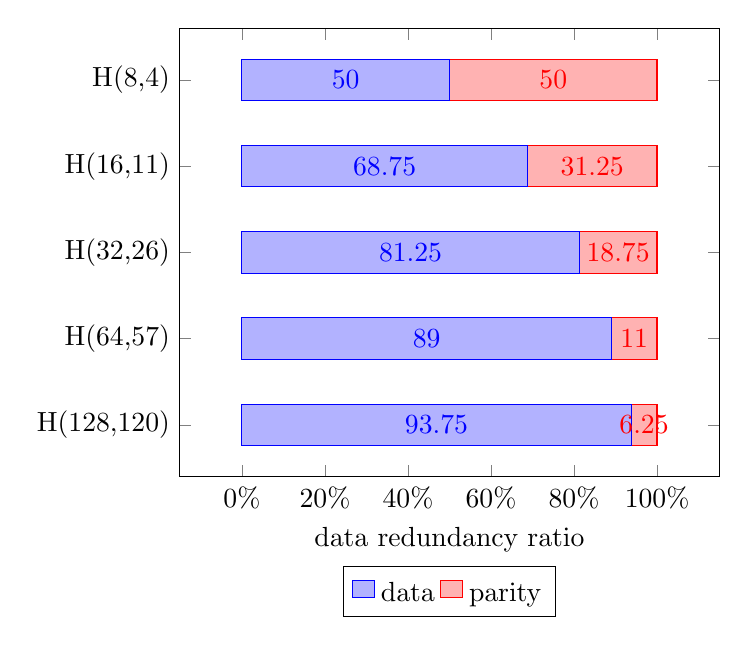
\begin{tikzpicture}
        \begin{axis}[
            xbar stacked,
            bar width=15pt,
            nodes near coords,
            enlargelimits=0.15,
            legend style={at={(0.5,-0.20)},
              anchor=north,legend columns=-1},
            xlabel={data redundancy ratio},
            symbolic y coords={H{(128,120)}, H{(64,57)}, H{(32,26)}, H{(16,11)}, H{(8,4)}},
            ytick=data,
            xmin=0,xmax=100,
            xticklabel={\pgfmathprintnumber{\tick}\%}
            ]
        \addplot+[xbar] plot coordinates {(93.75,H{(128,120)}) (89,H{(64,57)}) (81.25,H{(32,26)}) (68.75,H{(16,11)}) (50,H{(8,4)})};
        \addplot+[xbar] plot coordinates {(6.25,H{(128,120)}) (11,H{(64,57)}) (18.75,H{(32,26)}) (31.25,H{(16,11)}) (50,H{(8,4)})};
        \legend{\strut data, \strut parity}
        \end{axis}
    \end{tikzpicture}
    \label{fig:redundancyvsdata}
    \caption{Daten vs. Redundanz der unterschiedlichen Hamming-Codes}
\end{figure}